\documentclass{article}
\usepackage[utf8]{inputenc}
\usepackage[english]{babel}
 \usepackage{graphicx}
\graphicspath{ {.} }
\usepackage{multicol}
\special{papersize=8.5in,11in}
\usepackage[margin=0.8in]{geometry}
\usepackage{mathptmx}
\usepackage{lipsum}
\usepackage{amsmath}
\usepackage{amssymb}
\usepackage{enumitem}
\usepackage{fancyhdr}
\usepackage{mathtools}

\begin{document}

\noindent\LARGE{\textbf{On the effects of rotor wake turbulence on bat lungs and fish swim bladders}}
\vspace{0.3cm}
\normalsize

\hspace{0.5cm}Dorien Villafranco

\small\hspace{0.5cm}\textit{Department of Mechanical Engineering, Boston University, 110 Cummington Mall,}

\hspace{0.5cm}\textit{Boston, Massachusetts 02215}
\normalsize
\vspace{0.15cm}

\hspace{0.5cm}Jonathan Russell
\small

\hspace{0.5cm}\textit{Department of Mechanical Engineering, Boston University, 110 Cummington Mall,}

\hspace{0.5cm}\textit{Boston, Massachusetts 02215}

\normalsize
\vspace{8cm}
\begin{multicols}{2}
\noindent\textbf{I. INTRODUCTION}

\vspace{0.1cm}
This paper presents the effects of rotor wake turbulence on two animals, bats and fish, which are in constant contact with such turbulent distortions. It is known that bat mortality is increased near moving turbine blades usually found in wind farms (WFs). xx  Based on statistical data provided by WFs throughout the United States, it is predicted that as many as 110,000 bats may be killed on a yearly basis by 2020. xx Other authors disagree on this estimate, citing a much large number of 450,000 bats being killed per year by wind turbines in WFs throughout the country. xx. Despite the dispute surrounding the number of bats killed each year by wind turbines, it is clear that there exists a relationship between bat mortality and the operation of wind turbines. The issue is compounded by the fact that bats tend to have low reproductive rates. xx. As a result, even low levels of mortality can have a significant effect on the population of bats in a given region.

Zimmerling and Francis argue that the reason for the high mortality rate of bats in the vicinity of WFs is still uncertain. Behavior of bats at wind turbines have been studied and several suggestions are made as to reasons bats may gravitate toward wind turbines. It is suggested that near wind turbines, where the concentration of insects is high, bats would be drawn to the location as it is seen as a location abundant in food. It is also thought that bats may view the monopole of the turbine for a very tall tree. xx. All of these suggestions point to the fact that fatalities of bats near wind turbines may be the result of evolved advantageous behaviors prompted by tall trees but are now maladaptive when prompted by wind turbines.

The literature suggests two leading hypotheses for the mortality of bats in the vicinity of wind farms. It is supposed that the bats are either killed by direct contact with the turbine blades or by barotrauma. xx Barotrauma is an occurrence in which a sudden change in the surrounding air-pressure causes tissue damage to biological structures which contain air in the bat's body such as the lungs. A recent study has reported that barotrauma may be the cause for about 90$\%$ of bat deaths. The study demonstrates that the aforementioned proportion of bats were all found to have lesions associated with barotrauma. xx 

In spite of this, there exists opposition to bat barotrauma as a the major cause of death of bats near WFs. xx. It is therefore of interest to study further the effects wind turbines have on bat lungs. This computational study will provide further insight into the phenomenon by modeling the bat lung as spherical bubble with a visco-elastic shell. The encapsulation will then respond to pressure fields which are typical of WFs by importing such fields from OVERFLOW. This is a computational fluid dynamics (CFD) code which is able to simulate the wake of wind turbines and thus obtain pressure fields associated with their operation. Based on the reaction of the model lung, deductions will be made as to whether barotrauma is indeed a possible cause of death for bats in the vicinity of WFs. 

\vspace{25cm}
\noindent\textbf{II. LUNG MODEL}

\vspace{0.1cm}
In this study, both the bat lung and fish swim bladder will be modeled as gas bubble with an elastic solid surface layer. The model being used was developed by Church. In his work, a Rayleigh-Plesset-like equation is derived for the case of a spherical gas bubble which has a surface acting as a continuous, damped, elastic solid. Consider the spherical cavity shown below. The idealized depiction denotes the gas inside the bubble as G, the elastic shell as S and the unbounded liquid free of body forces which the cavity is immersed in as L. \\

\hspace{1.8cm}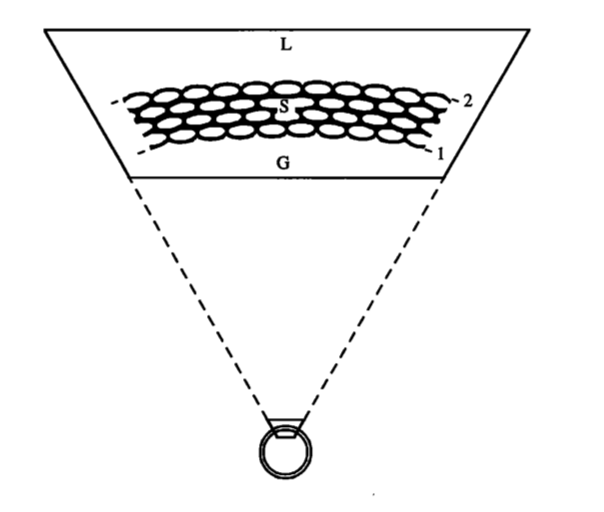
\includegraphics[scale = 0.2]{Model_Bubble}\\
\small\textbf{Figure 1}: Depiction of gas bubble with surface layer of elastic solid, with inner and outer radius 1, and 2 respectively immersed in liquid
\normalsize

\begin{equation*}
R_1U_1 \Bigg[1+ \Bigg(\frac{\rho_L - \rho_S}{\rho_S}\Bigg)\frac{R_1}{R_2}\Bigg] 
+ U_1^2\Bigg[\frac{3}{2} + \Bigg(\frac{\rho_L - \rho_S}{\rho_S}\Bigg)\times \Bigg(\frac{4R_2^3 - R_1^3}{2R_2^3}\Bigg)\frac{R_1}{R_2}\Bigg] 
\end{equation*}
\begin{equation*}
= \frac{1}{\rho_S}\Bigg[P_{G,eq}\Bigg(\frac{R_{01}}{R_1}\Bigg)^{4\kappa} - P_\infty(t) - \frac{2\sigma_1}{R_1}-\frac{2\sigma_2}{R_2}
\end{equation*}
\begin{equation*}
 - 4\frac{U_1}{R_1}\Bigg(\frac{V_S \mu_S + R_1^3 \mu_L}{R_2^3}\Bigg) - 4 \frac{V_SG_S}{R_2^3}\Bigg(1 - \frac{R_{e1}}{R_1}\Bigg)\Bigg]
\end{equation*}
where $V_S = R^2_{02} - R^3_{01}$


\newpage

\end{multicols}
\end{document}